\chapter{आहार शृंखलाएँ}\label{ch:g3:food-chains}

मैदान में घास उगती है। एक टिड्डा घास खाता है। एक छिपकली टिड्डे को पकड़
लेती है। ऊपर मँडराता एक बाज़ छिपकली को उठा ले जाता है। चार भोजन --- और
अचानक बाज़ की दोपहर इस पर निर्भर हो जाती है कि घास कितनी हरी उगी।
प्रकृति के भोजन शृंखलाओं में जुड़ जाते हैं, और उन्हें पढ़ना सीखना यह
सीखना है कि पूरा मैदान कैसे आपस में बँधा हुआ है।

\section{आहार शृंखला पढ़ना और लिखना}

\begin{definition}[आहार शृंखला]\label{def:g3:food-chains:chain}
\emph{आहार शृंखला}\index{आहार शृंखला} सजीवों की वह क़तार है जिसमें हर
एक को अगला खा जाता है। इसे तीरों से लिखा जाता है, और हर तीर का अर्थ है
\emph{``द्वारा खाया जाता है''}\index{द्वारा खाया जाता है}:
\[
\text{घास} \longrightarrow \text{टिड्डा}
\longrightarrow \text{छिपकली} \longrightarrow \text{बाज़}.
\]
हर \omterm{def:g1:living-or-not:living}{सजीव} शृंखला की एक \emph{कड़ी}\index{कड़ी} है।
\end{definition}

\begin{remark}[तीर की दिशा का ध्यान रखो]\label{rem:g3:food-chains:arrow}
तीर खाए जाने वाले से खाने वाले की ओर जाता है --- वह भोजन के पीछे चलता
है। ``घास $\rightarrow$ टिड्डा'' पढ़ा जाता है ``घास टिड्डे द्वारा खाई
जाती है''। तीर उलटे लिखना --- यानी खाने की ओर --- \omterm{def:g3:food-chains:chain}{आहार शृंखलाओं} की सबसे
आम ग़लती है; याद रखो कि तीर दिखाता है कि भोजन \emph{कहाँ जाता है}।
\end{remark}

\begin{proposition}[हर शृंखला किसी पौधे से शुरू होती है]\label{prop:g3:food-chains:start}
\omterm{def:g3:food-chains:chain}{आहार शृंखला} की पहली कड़ी हमेशा कोई \omterm{def:g1:plants-around-us:plant}{पौधा} होता है (या कोई और \omterm{def:g1:living-or-not:living}{सजीव} जो
अपना भोजन ख़ुद बनाता है)। सिर्फ़ \omterm{def:g1:plants-around-us:plant}{पौधे} ही किसी को खाए बिना पोषण लेते हैं
--- प्रकाश, पानी और हवा से, जैसा \cref{def:g1:plants-around-us:plant}
ने कहा था। हर जंतु-कड़ी सीधे या दूसरों के ज़रिए उसी पहली हरी कड़ी पर
जीती है।
\end{proposition}
\admitted

\begin{example}[तीन आवासों की शृंखलाएँ]\label{ex:g3:food-chains:three}
तालाब में: पानी के \omterm{def:g1:plants-around-us:plant}{पौधे} $\rightarrow$ \omterm{ex:g2:animals-grow-up:frog}{टैडपोल} $\rightarrow$
व्याध-पतंगे का डिंभ $\rightarrow$ काँटा-मछली $\rightarrow$ बगुला।
जंगल में: बलूत की \omterm{def:g1:plants-around-us:parts}{पत्तियाँ} $\rightarrow$ \omterm{ex:g2:animals-grow-up:butterfly}{इल्ली} $\rightarrow$ नीली
चिड़िया $\rightarrow$ बाज़। बग़ीचे में: सलाद $\rightarrow$ घोंघा
$\rightarrow$ साही। पहली कड़ी: हमेशा हरी।
\end{example}

\begin{omfigure}
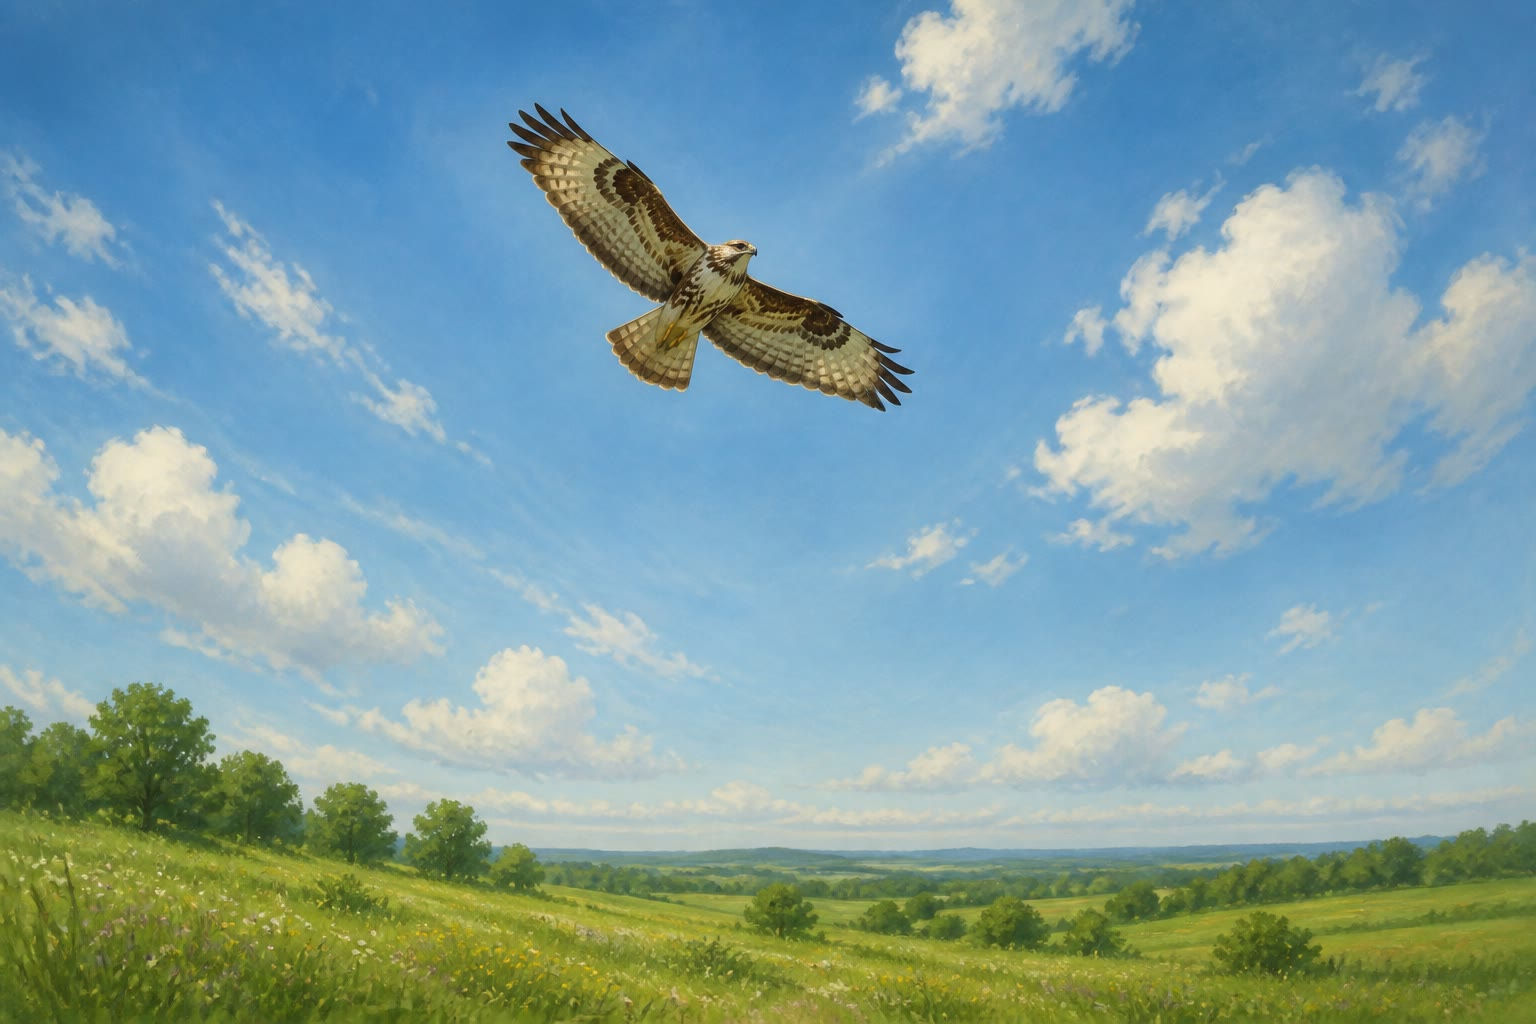
\includegraphics[width=0.6\linewidth]{images/book1/ai/g3-chains-buzzard.jpg}

{\small मैदान की शृंखला की आख़िरी कड़ी गश्त पर: बाज़ की दोपहर, तीन
कड़ियाँ नीचे, इस बात पर निर्भर है कि घास कितनी हरी उगी।}
\end{omfigure}

\begin{method}[आहार शृंखला बनाना]\label{met:g3:food-chains:build}
\begin{enumerate}
  \item कोई \omterm{def:g1:animals-around-us:animal}{जंतु} चुनो और पूछो: वह क्या खाता है? भोजन को उसकी बाईं ओर
        लिखो, और तीर खाने वाले की ओर;
  \item वही सवाल उस भोजन से पूछो, और बाईं ओर तब तक बढ़ते जाओ जब तक
        कोई \omterm{def:g1:plants-around-us:plant}{पौधा} न मिल जाए;
  \item पूछो: मेरे शुरू वाले \omterm{def:g1:animals-around-us:animal}{जंतु} को कौन खाता है? जब तक कोई खाने वाला
        हो, दाईं ओर बढ़ाते जाओ;
  \item जाँचो कि हर तीर \omterm{def:g3:food-chains:chain}{``द्वारा खाया जाता है''} पढ़ा जाता है --- यानी
        भोजन दाईं ओर बहता है।
\end{enumerate}
\end{method}

\section{जब कोई कड़ी बदलती है}

\begin{proposition}[कड़ियाँ एक-दूसरे पर निर्भर हैं]\label{prop:g3:food-chains:depend}
\omterm{def:g3:food-chains:chain}{आहार शृंखला} में हर कड़ी अपने से पहले वालों पर निर्भर है, और अपने से बाद
वालों का पोषण करती है। कोई एक कड़ी कम हो जाए तो अगली कड़ियाँ भूखी रह
जाती हैं --- और उससे \emph{पहले} वाली कड़ी, अब उतनी न खाई जाने के कारण,
बढ़ सकती है। एक कड़ी का बदलाव पूरी शृंखला में सफ़र करता है।
\end{proposition}
\admitted

\begin{example}[सूखी गर्मी]\label{ex:g3:food-chains:dry}
सूखे से मैदान की घास भूरी पड़ जाती है। भोजन की कमी से टिड्डे कम रह जाते
हैं; उनका शिकार करने वाली छिपकलियाँ भूखी रहती हैं और अपनी बारी में
बाज़ का पोषण भी ठीक से नहीं कर पातीं। पहली कड़ी भूरी पड़ी, और उसके ऊपर
की पूरी शृंखला पतली हो गई --- बाज़ ने घास कभी नहीं खाई, फिर भी उसे सूखा
महसूस होता है।
\end{example}

\begin{example}[शिकारी को हटाना]\label{ex:g3:food-chains:hunter}
मान लो घाटी से बाज़ ग़ायब हो जाते हैं। कम शिकार होने से छिपकलियाँ बढ़
जाती हैं; तब टिड्डे ज़्यादा खाए जाते हैं और घट जाते हैं; और घास, कम
कुतरी जाने से, शायद और घनी हो जाए। \emph{आख़िरी} कड़ी हटाना भी शृंखला
में सफ़र करता है --- बस दूसरी दिशा में।
\end{example}

\begin{remark}[असली मैदान जाल होते हैं]\label{rem:g3:food-chains:web}
हमारी शृंखला एक अकेला धागा है, पर बाज़ चूहे भी उठाता है, छिपकली
मक्खियाँ भी खाती है, और घास ख़रगोशों का भी पोषण करती है। कई शृंखलाएँ
आपस में कटकर एक जाल बनाती हैं --- वही \emph{आहार जाल} जिसे आगे का एक
साल पढ़ेगा (\cref{ch:g2:what-animals-eat} ने लोमड़ी, ख़रगोश और घास से
इसका इशारा दे ही दिया था)। पहले शृंखलाएँ: वे ही वे धागे हैं जिनसे जाल
बुना जाता है।
\end{remark}

\section{अभ्यास}

\begin{exercise}[$\star$]\label{exo:g3:food-chains:1}
\omterm{def:g3:food-chains:chain}{आहार शृंखला} के तीर का क्या अर्थ है? वह किस ओर इशारा करता है?
\end{exercise}

\begin{exercise}[$\star$]\label{exo:g3:food-chains:2}
पहली कड़ी हमेशा किस तरह का \omterm{def:g1:living-or-not:living}{सजीव} होता है? क्यों?
\end{exercise}

\begin{exercise}[$\star$]\label{exo:g3:food-chains:3}
इस अध्याय की मैदान वाली शृंखला उसकी चारों कड़ियों और तीरों के साथ
लिखो।
\end{exercise}

\begin{exercise}[$\star$]\label{exo:g3:food-chains:4}
इस शृंखला को ठीक करो: लोमड़ी $\rightarrow$ ख़रगोश $\rightarrow$
घास।
\end{exercise}

\begin{exercise}[$\star$]\label{exo:g3:food-chains:5}
इन कड़ियों से एक शृंखला बनाओ: नीली चिड़िया, बलूत की \omterm{def:g1:plants-around-us:parts}{पत्तियाँ}, बाज़,
\omterm{ex:g2:animals-grow-up:butterfly}{इल्ली}।
\end{exercise}

\begin{exercise}[$\star$]\label{exo:g3:food-chains:6}
बग़ीचे की शृंखला सलाद $\rightarrow$ घोंघा $\rightarrow$ साही में,
घोंघा किसे खा जाता है? घोंघे को कौन खाता है?
\end{exercise}

\begin{exercise}[$\star$]\label{exo:g3:food-chains:7}
\cref{met:g3:food-chains:build} से कम से कम तीन कड़ियों की एक शृंखला
बनाओ, जो तालाब के बगुले पर ख़त्म हो।
\end{exercise}

\begin{exercise}[$\star$]\label{exo:g3:food-chains:8}
\cref{ex:g3:food-chains:dry} की सूखी गर्मी में बाज़ को तकलीफ़ क्यों
होती है, जबकि वह घास कभी नहीं खाता?
\end{exercise}

\begin{exercise}[$\star\star$]\label{exo:g3:food-chains:9}
जो माली हर घोंघे को ज़हर देते हैं वे कभी-कभी अपना साही खो बैठते हैं ---
और फिर उन्हें पहले से \emph{ज़्यादा} स्लग और घोंघे मिलते हैं। दोनों
बातें \cref{prop:g3:food-chains:depend} से समझाओ।
\end{exercise}

\begin{exercise}[$\star\star$]\label{exo:g3:food-chains:10}
``छिपकली घास पर निर्भर है।'' सही या ग़लत? मैदान की शृंखला से अपने उत्तर
का बचाव करो --- और बताओ कि घास की कमी किस दिशा में सफ़र करती है।
\end{exercise}
